\subsection*{Assignment2.b \hrule}
\textbf{Question}
\begin{quote}
Make a log-log plot of and plot single points for $n(10^{-4})$, $n(10^{-2})$, $n(10^{-1}$), $n(1)$ and $n(5)$ with an axis range from $x = 10^{-4}$ to $x_{max} = 5$. Interpolate the values in between based on just these points - make sure to argue in the comments of your code why you chose to interpolate in a certain way.
\end{quote}

\textbf{Solution}
\begin{quote}
Four out of the 5 points plotted in logarithmic space seems to follow a straight line (see figure 3 below the code section). If we assume that the error on these points is small, then this suggests that the underlying physical relation might be a linear relation in logarithmic space. The last point deviates from this relation with a rapid drop. If we again assume that the error is small, then this suggests that there might be an exponential decrease. 


Most of the data seems to follow a linear relation in log space. If you need to interpolate a value, then you likely need to interpolate withing this linear part, as it wouldn't make much sense to obtained most of your data in a region that is uninteresting. An interpolator should furthermore serve the data  as best as possible. Interpolating the data with a linear and for example a polynomial interpolator, shows that the polynomial interpolator better interpolates the expected exponential drop, where as the linear interpolator better interpolates the expected power law (see figure 4 below the code section). Many other interpolation methods, such as cubic splines and nearest neighbor interpolation, also interpolate the expected exponential drop better than the linear interpolator, but fail to interpolate the linear relation with high accuracy (not shown). 

Based on the above two arguments there is therefore chosen to interpolate the points with a \textbf{linear interpolate} in log space. 


  
The code for this assignment consists of two files: \textsf{./code/assignment2\_ b.py} and   \textsf{./code/mathlib/interpolate.py}. The first file creates the plots and the second file implements the interpolation methods. The code of the two files and the results can be found below.
\newpage
\end{quote}


\textbf{Code - output}
\begin{quote}
The code that interpolates the values and creates the plot.
\lstinputlisting{./code/assignment2_b.py}
\end{quote}

\textbf{Code - interpolate}
\begin{quote}
The code of the linear and polynomial interpolator.
\lstinputlisting{./code/mathlib/interpolate.py}
\end{quote}
\newpage

\textbf{Output - Figure}
\begin{quote}
\begin{figure}[!ht]
\centering
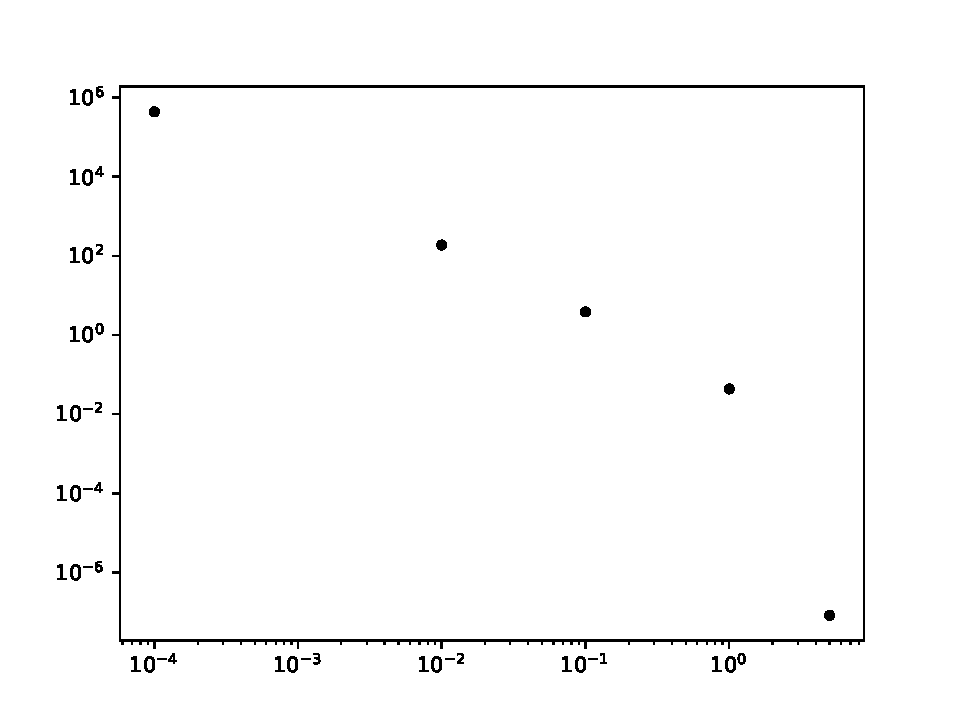
\includegraphics[scale=0.7]{plots/points.pdf}
\caption{A logarithmic plot of the 5 points that need to be interpolated.}
\end{figure}

\begin{figure}[!ht]
\centering
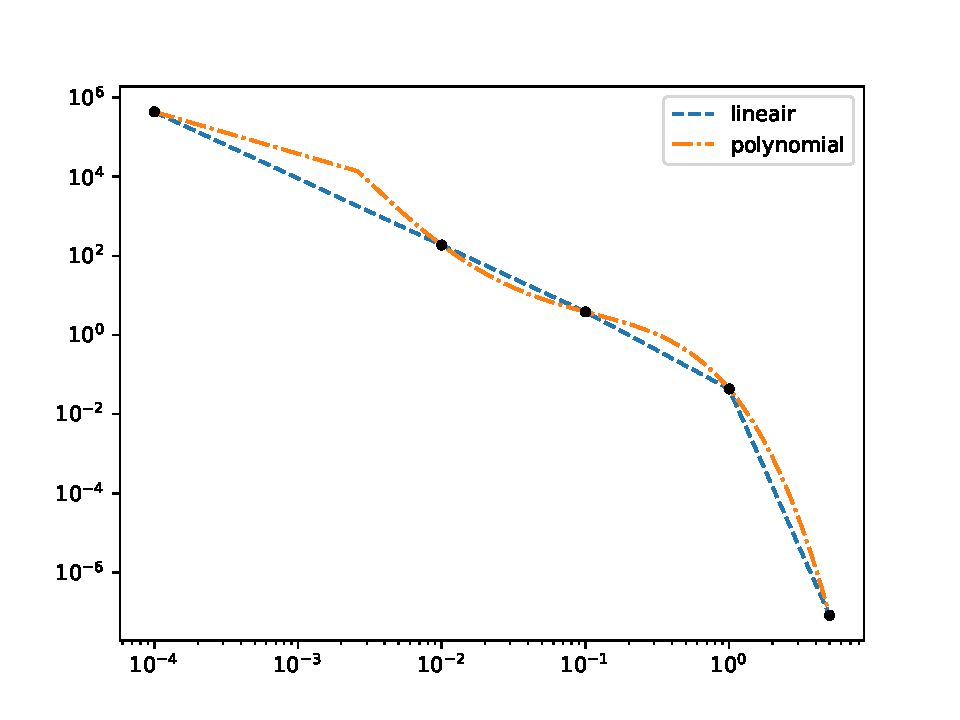
\includegraphics[scale=0.7]{plots/interpolate.pdf}
\caption{The interpolation of the linear interpolator and the polynomial interpolator.}
\end{figure}
\end{quote}
\newpage


 









